\documentclass[12pt]{article}

% 基础宏包
\usepackage{graphicx}  % 插入图片
\usepackage[english]{babel}  % 英语语言支持
% \usepackage[UTF8]{ctex}  % 如果不需要中文，可以注释掉这一行

% 数学宏包
\usepackage{amsmath}  % 数学排版增强
\usepackage{amsfonts} % 数学字体

% 图表相关
\usepackage{float}    % 浮动体控制 [H] 选项
\usepackage{tikz}     % 绘图
\usepackage{pgfplots} % 函数绘图
\pgfplotsset{compat=1.18} % 设置pgfplots兼容性

% 页面设置
\usepackage{geometry}
\geometry{
  a4paper,
  left=2cm,
  right=2cm,
  top=2cm,
  bottom=2cm
}

% 版式设置
\usepackage{fancyhdr}    % 页眉页脚
\usepackage{lastpage}    % 最后一页引用
\usepackage{multicol}    % 多栏排版
\usepackage{tabularx}    % 表格增强

% 文本修饰
\usepackage{ulem}        % 下划线等
\usepackage{enumitem}    % 列表样式
\usepackage{titlesec}    % 标题样式
\usepackage[export]{adjustbox} % 图片对齐

% 颜色
\usepackage{color}       % 颜色支持

\linespread{1.5}         % 1.5倍行距

\title{Lab 1}
\author{Emilien Zhang}
\date{17 March 2026}

\begin{document}

\maketitle

\section*{Problem 1}

\begin{figure}[H]
  \centering
  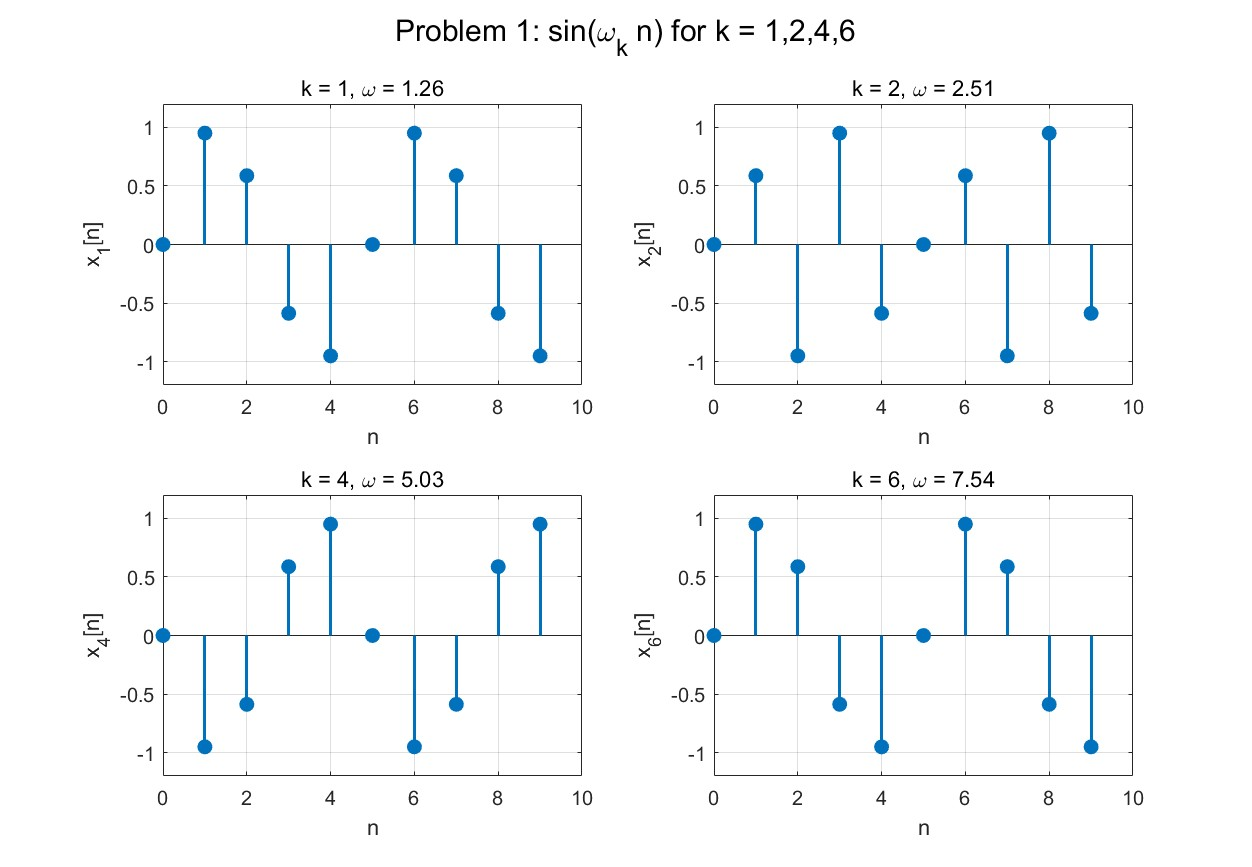
\includegraphics[width=1.0\textwidth]{1.jpg}
  \caption{Figure for problem 1}
  \label{fig1}
\end{figure}

In Figure~\ref{fig1}, we plotted the signals $x_k[n] = \sin\left(\dfrac{2\pi k}{5}n\right)$ for $k = 1, 2, 4, 6$ respectively. We observed three unique signals (for $k = 1, 2, 4$). The plots for $k = 1$ and $k = 6$ are identical because the sine function is periodic with period $2\pi$. 

For a periodic signal $x(t)$ with a fundamental period $T$, we have
\[
x(t + nT) = x(t)
\]
where $n$ is an integer.

In this problem, it is clear that
$$x_{k=6}[n]=\sin\left(\frac{12\pi}{5}n\right)=\sin\left(\frac{2\pi}{5}n+2n\pi\right)=\sin\left(\frac{2\pi}{5}n\right)=x_{k=1}[n].$$
This explains why different values of $k$ can yield the same signal.

\section*{Problem 2}

\begin{figure}[H]
  \centering
  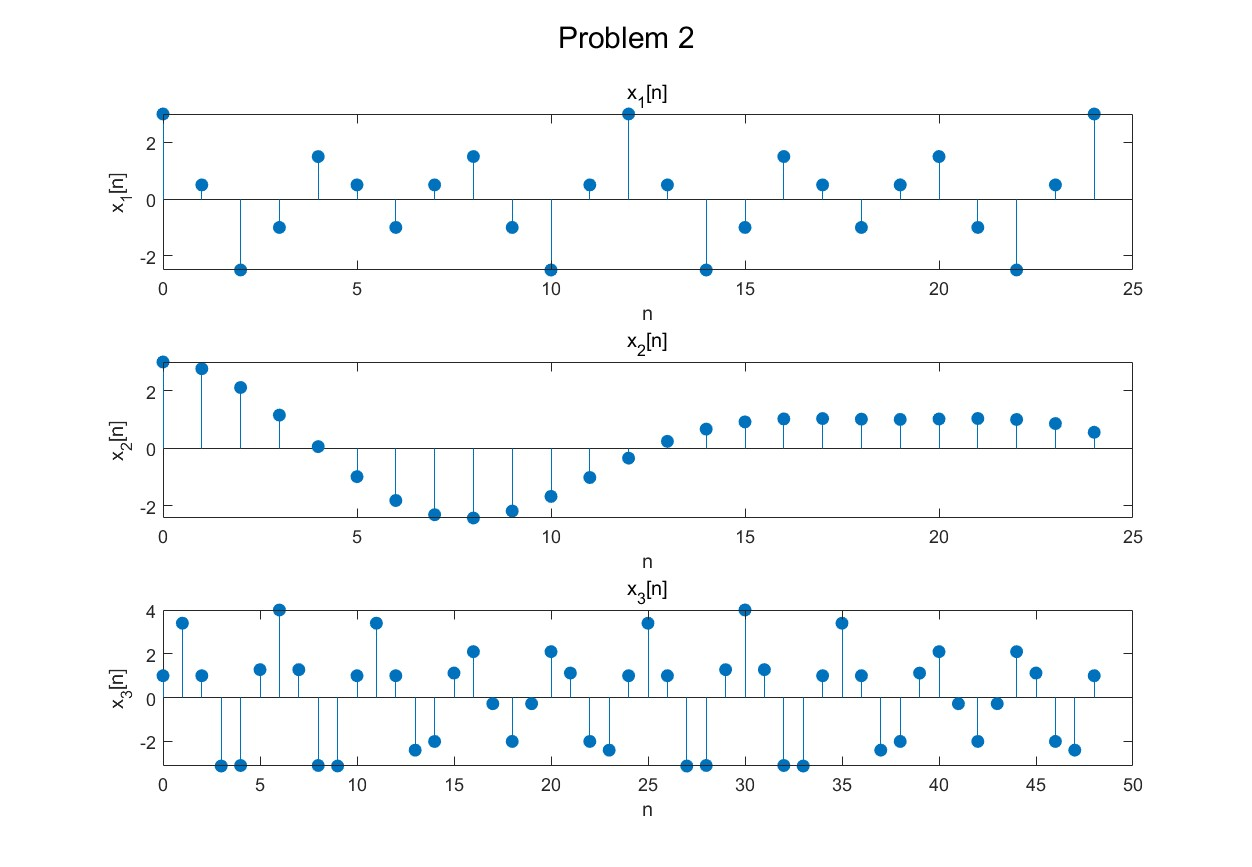
\includegraphics[width=1.0\textwidth]{2.jpg}
  \caption{Figure for problem 2}
  \label{fig2}
\end{figure}

For \(N = 6\):

\begin{itemize}
  \item \(x_1[n] = \cos\left(\dfrac{2\pi n}{6}\right) + 2\cos\left(\dfrac{3\pi n}{6}\right) = \cos\left(\dfrac{\pi n}{3}\right) + 2\cos\left(\dfrac{\pi n}{2}\right)\).
  The periods of the two components are \(T_1 = 6\) and \(T_2 = 4\). The fundamental period is \(\text{lcm}(6,4) = 12\). Therefore, \(x_1[n]\) is periodic with period 12.
  
  \item \(x_2[n] = 2\cos\left(\dfrac{2n}{6}\right) + \cos\left(\dfrac{3n}{6}\right) = 2\cos\left(\dfrac{n}{3}\right) + \cos\left(\dfrac{n}{2}\right)\).
  Here \(\omega_1 = 1/3\) and \(\omega_2 = 1/2\). For a discrete-time signal to be periodic, we need \(\dfrac{\omega_1}{2\pi} = \dfrac{1}{6\pi}\) and \(\dfrac{\omega_2}{2\pi} = \dfrac{1}{4\pi}\) to be rational numbers. Since \(1/(6\pi)\) is not rational, \(x_2[n]\) is \textbf{not periodic}.
  
  \item \(x_3[n] = \cos\left(\dfrac{2\pi n}{6}\right) + 3\sin\left(\dfrac{5\pi n}{12}\right) = \cos\left(\dfrac{\pi n}{3}\right) + 3\sin\left(\dfrac{5\pi n}{12}\right)\).
  The periods are \(T_1 = 6\) for the cosine term, and for the sine term we have \(\omega = 5\pi/12\), so \(\dfrac{\omega}{2\pi} = \dfrac{5}{24}\), which is rational. Thus the period of the sine term is \(T_2 = 24\). The fundamental period is \(\text{lcm}(6,24) = 24\). Therefore, \(x_3[n]\) is periodic with period 24.
\end{itemize}

\section*{Problem 3}

\begin{figure}[H]
  \centering
  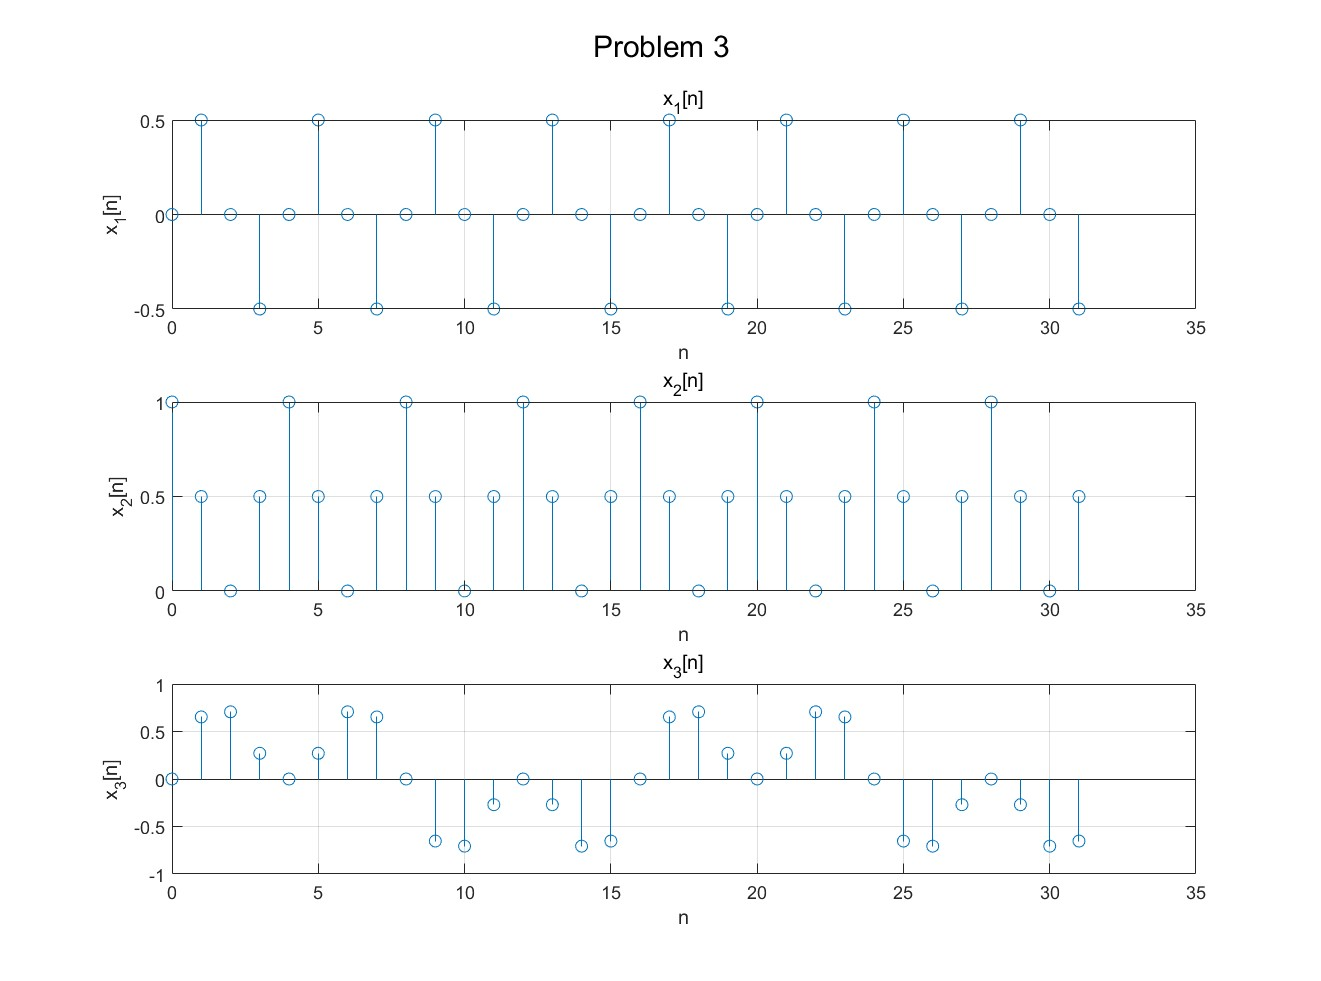
\includegraphics[width=1.0\textwidth]{3.jpg}
  \caption{Figure for problem 3}
  \label{fig3}
\end{figure}

Using trigonometric identities:
\begin{align*}
x_1[n] &= \sin\left(\frac{\pi n}{4}\right)\cos\left(\frac{\pi n}{4}\right) = \frac{1}{2}\sin\left(\frac{\pi n}{2}\right), \\
x_2[n] &= \cos^2\left(\frac{\pi n}{4}\right) = \frac{1}{2}\left[1 + \cos\left(\frac{\pi n}{2}\right)\right], \\
x_3[n] &= \sin\left(\frac{\pi n}{4}\right)\cos\left(\frac{\pi n}{8}\right) = \frac{1}{2}\left[\sin\left(\frac{3\pi n}{8}\right) + \sin\left(\frac{\pi n}{8}\right)\right].
\end{align*}

The fundamental periods are:
\begin{itemize}
  \item For \(x_1[n]\): \(\omega = \pi/2\), so \(T = \dfrac{2\pi}{\pi/2} = 4\).
  \item For \(x_2[n]\): The constant term does not affect periodicity; the cosine term has \(\omega = \pi/2\), so \(T = 4\).
  \item For \(x_3[n]\): The two components have frequencies \(\omega_1 = 3\pi/8\) and \(\omega_2 = \pi/8\). Their periods are \(T_1 = \dfrac{2\pi}{3\pi/8} = \dfrac{16}{3}\) and \(T_2 = \dfrac{2\pi}{\pi/8} = 16\). Since the period must be an integer, the fundamental period is determined by the least common multiple of the denominators when expressed in rational form. Here, \(\dfrac{\omega_1}{2\pi} = \dfrac{3}{16}\) and \(\dfrac{\omega_2}{2\pi} = \dfrac{1}{16}\), both rational, so the fundamental period is \(T = \text{lcm}(16,16) = 16\).
\end{itemize}

\section*{Problem 4}

The sum of two periodic signals is \textbf{not necessarily periodic}. For \(x[n] = x_1[n] + x_2[n]\) to be periodic, the periods \(T_1\) and \(T_2\) must have a common multiple (i.e., \(T_1/T_2\) must be rational). If the ratio of periods is irrational, the sum is not periodic, as seen in Problem 2 with \(x_2[n]\).

The product of two periodic signals is also \textbf{not necessarily periodic}. Using trigonometric identities, multiplication can be expressed as sums of sinusoids with frequencies that are sums and differences of the original frequencies. The resulting signal is periodic if and only if the ratio of all resulting frequency components to \(2\pi\) is rational, which is not guaranteed even if the original signals are periodic.

\section*{Problem 5}

\begin{figure}[H]
  \centering
  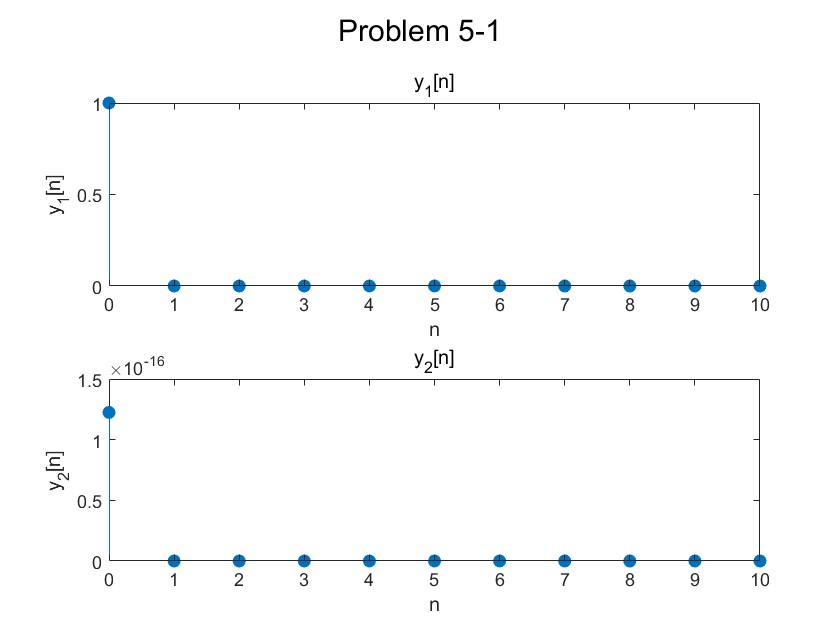
\includegraphics[width=0.7\textwidth]{4.jpg}
  \caption{Figure for problem 5-1}
  \label{fig4}
\end{figure}

The system \( y[n] = \sin((\pi/2)x[n]) \) is nonlinear. To demonstrate this, we use the signals \( x_1[n] = \delta[n] \) and \( x_2[n] = 2\delta[n] \).

For a linear system, the principle of superposition must hold:
\[
T\{a x_1[n] + b x_2[n]\} = a T\{x_1[n]\} + b T\{x_2[n]\}
\]

Let's compute the responses:

For \( x_1[n] = \delta[n] \):
\[
y_1[n] = \sin\left(\frac{\pi}{2} \delta[n]\right) = 
\begin{cases}
\sin(\pi/2) = 1, & n = 0 \\
\sin(0) = 0, & n \neq 0
\end{cases}
\]
So \( y_1[n] = \delta[n] \).

If the system were linear, the response to \( x_2[n] = 2\delta[n] \) should be \( 2\delta[n] \).

However, the actual output for the input \( 2\delta[n] \) is:
\[
y_2[n] = \sin\left(\frac{\pi}{2} \cdot 2\delta[n]\right) = \sin(\pi \delta[n]) = 
\begin{cases}
\sin(\pi) = 0, & n = 0 \\
\sin(0) = 0, & n \neq 0
\end{cases}
\]
So \( y_2[n] = 0 \) for all \( n \), not \( 2\delta[n] \). Therefore, the system is nonlinear.

\begin{figure}[H]
  \centering
  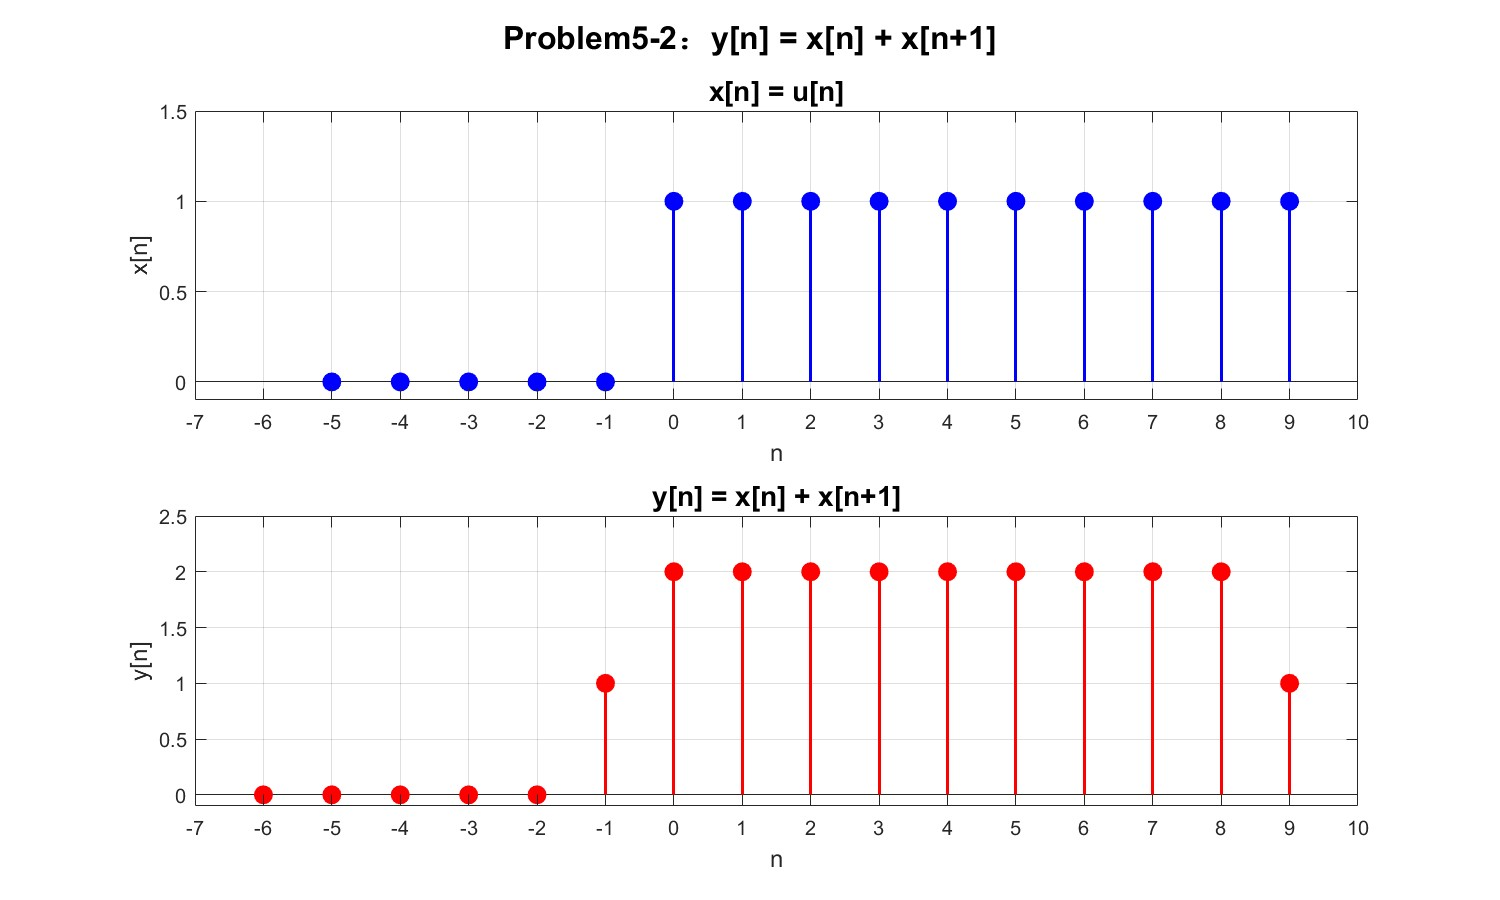
\includegraphics[width=0.8\textwidth]{5.jpg}
  \caption{Figure for problem 5-2}
  \label{fig5}
\end{figure}

The system \( y[n] = x[n] + x[n+1] \) is not causal because the output at time \( n \) depends on the input at time \( n+1 \) (a future value). As shown in Figure~\ref{fig5}, the output signal starts at \( n = -1 \), while the input signal starts at \( n = 0 \). This demonstrates that the system requires future input values to compute the output, confirming its non-causality.

\section*{Problem 6}

\begin{figure}[H]
  \centering
  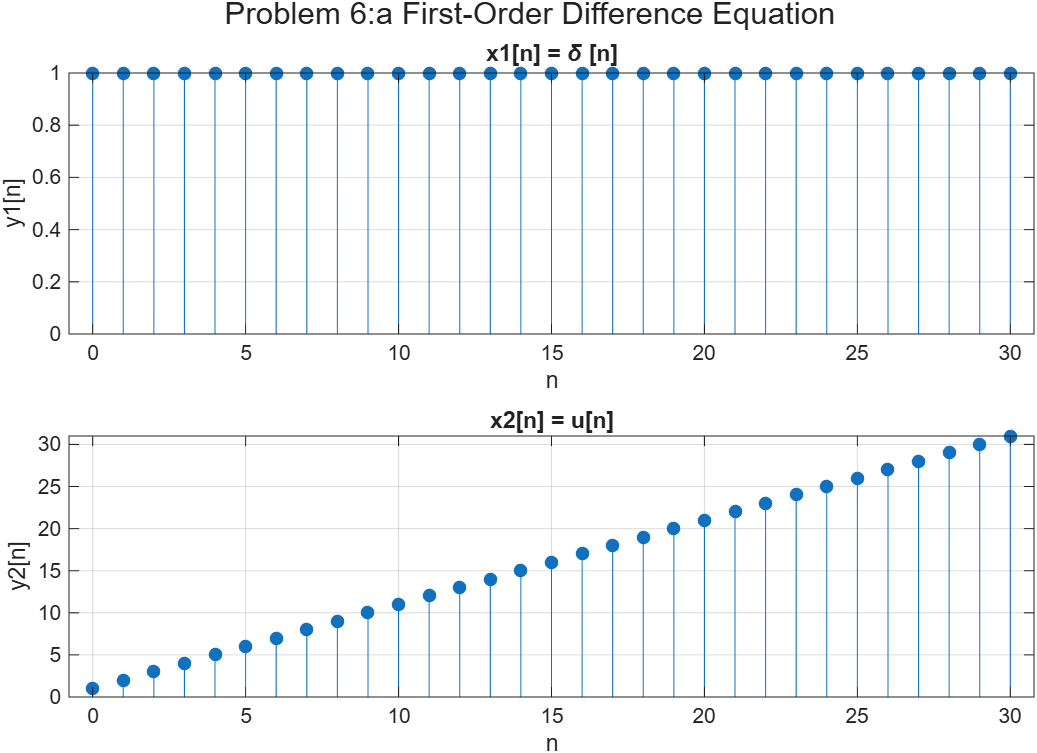
\includegraphics[width=0.8\textwidth]{6.png}
  \caption{Figure for problem 6}
  \label{fig6}
\end{figure}

The system is described by the difference equation:
$$y[n] = a y[n-1] + x[n]$$

For \(a = 1\) and \(y[-1] = 0\), this becomes:
$$y[n] = y[n-1] + x[n]$$

\begin{itemize}
  \item For \(x_1[n] = \delta[n]\): 
  \(y[0] = 1 \cdot 0 + 1 = 1\), and for \(n \geq 1\), \(y[n] = y[n-1] + 0\), so \(y[n] = 1\) for all \(n \geq 0\).
  
  \item For \(x_2[n] = u[n]\): 
  \(y[0] = 1 \cdot 0 + 1 = 1\), and for \(n \geq 1\), \(y[n] = y[n-1] + 1\), so \(y[n] = n + 1\).
\end{itemize}

We can observe that this system acts as a discrete-time accumulator (summator).

\section*{Problem 7}

\begin{figure}[H]
  \centering
  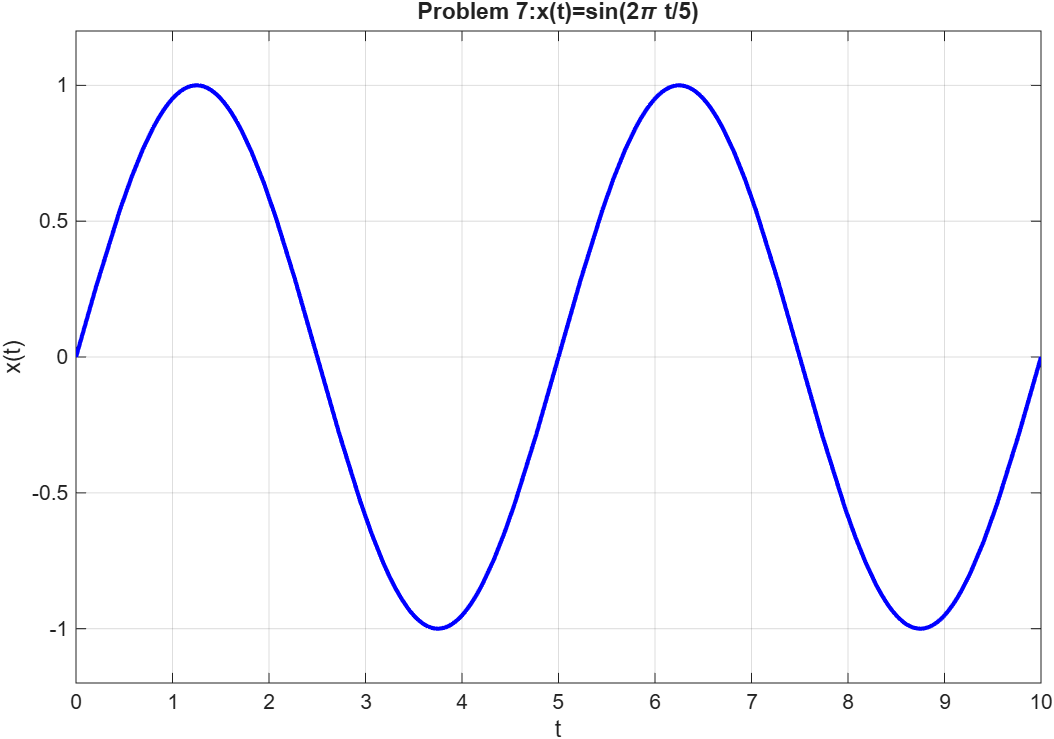
\includegraphics[width=0.6\textwidth]{7.png}
  \caption{Figure for problem 7}
  \label{fig7}
\end{figure}

Using MATLAB's symbolic toolbox, we create the symbolic expression for \(x(t) = \sin(2\pi t/5)\) and plot two periods:

\begin{verbatim}
>> x = sym('sin(2*pi*t/5)');
>> ezplot(x, [0, 10]);
>> xlabel('t');
>> ylabel('sin(2\pi t/5)');
>> title('Two periods of sin(2\pi t/5)');
\end{verbatim}

The plot shows two complete periods of the sinusoid from \(t = 0\) to \(t = 10\), since the fundamental period is \(T = 5\).

\section*{Problem 8}

\begin{figure}[H]
  \centering
  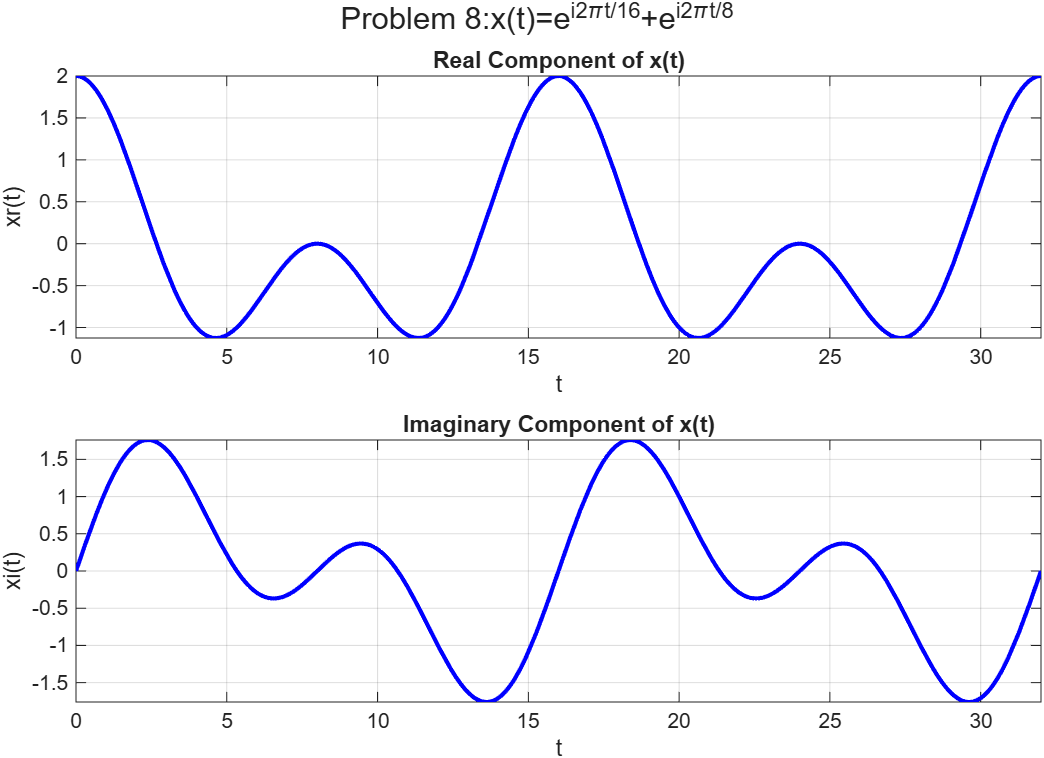
\includegraphics[width=0.8\textwidth]{8.png}
  \caption{Figure for problem 8}
  \label{fig8}
\end{figure}

Using Euler's formula, we have:
$$x(t) = e^{i2\pi t/16} + e^{i2\pi t/8} = \cos\frac{\pi t}{8} + i\sin\frac{\pi t}{8} + \cos\frac{\pi t}{4} + i\sin\frac{\pi t}{4}$$
$$= \left[\cos\frac{\pi t}{8} + \cos\frac{\pi t}{4}\right] + i\left[\sin\frac{\pi t}{8} + \sin\frac{\pi t}{4}\right]$$

So the real and imaginary components of the signal are:
$$\operatorname{Re}[x(t)] = \cos\frac{\pi t}{8} + \cos\frac{\pi t}{4}$$
$$\operatorname{Im}[x(t)] = \sin\frac{\pi t}{8} + \sin\frac{\pi t}{4}$$

The periods of the individual components are 16 and 8 respectively. Since 8 divides 16, the fundamental period of the overall signal is 16.

Therefore, \(x(t)\) is periodic with period \(T = 16\).

\end{document}